\section{The Robot Software System (LabVIEW)}

\subsection{The FPGA Hindbrain}
As discussed in the software overview section, the Hindbrain of the vehicle is implemented on a LabVIEW FPGA in order to ensure that control loops and essential data processing is done at the fastest possible speeds to reduce system latency even when the vehicle travels at higher speeds. \\ \\
%
The front panel and block diagram of the top-level hindbrain VI is shown below:

\begin{figure}[h!]
\centering
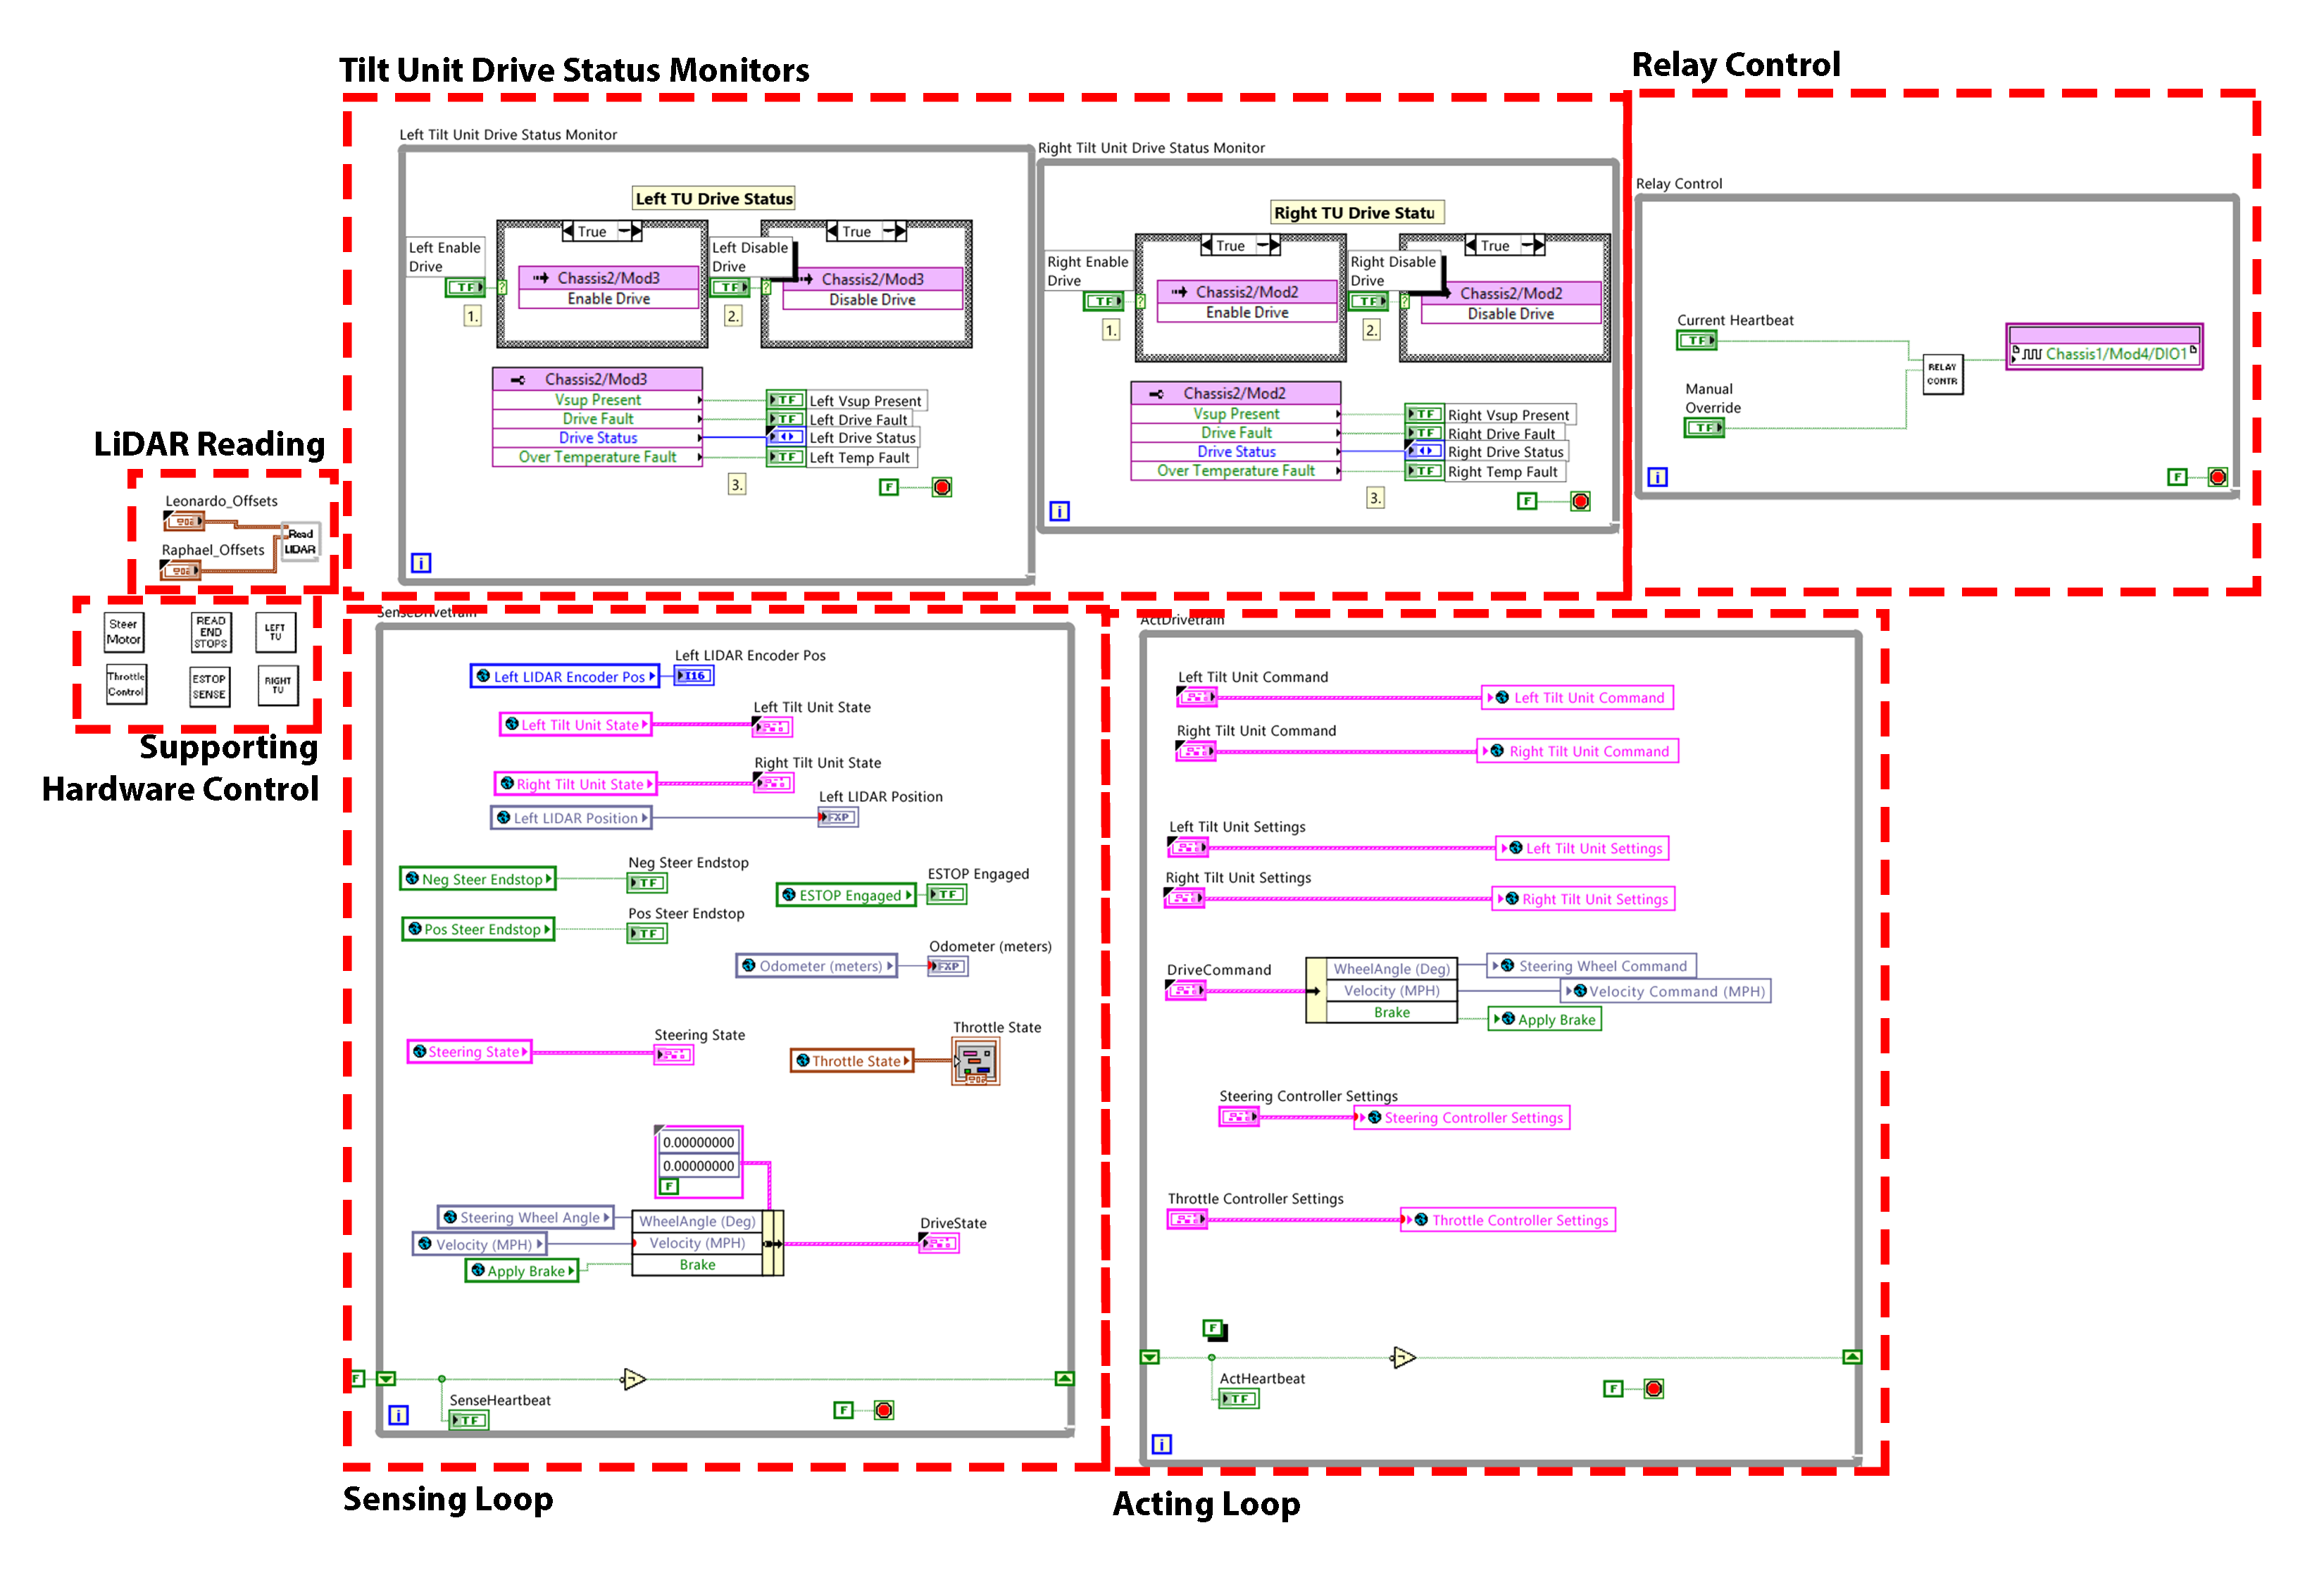
\includegraphics[scale=0.55]{Photos/hindbrainblock_annotated.png}
\caption{Hindbrain top-level VI block diagram with subsections annotated}
\label{fig:hindbrainblock}
\end{figure} 

\newpage

\noindent As can be seen in Figure \ref{fig:hindbrainblock}, the main subsections of the FPGA hindbrain are:

\begin{enumerate}
\item Sensing Loop
\item Acting Loop
\item Tilt Unit Drive Status Monitors
\item LiDAR Reading
\item Supporting Hardware Control
\item Relay Control
\end{enumerate}

\subsubsection{Sensing Loop}

The sensing loop of the FPGA hindbrain essentially passes status information and data from other parts of the FPGA hindbrain code up to the front panel so that the real-time code can access these variables. The block diagram for the sensing loop shown in Figure \ref{fig:hindbrainblock} is shown zoomed in below: 

\newpage

\begin{figure}[h!]
\centering
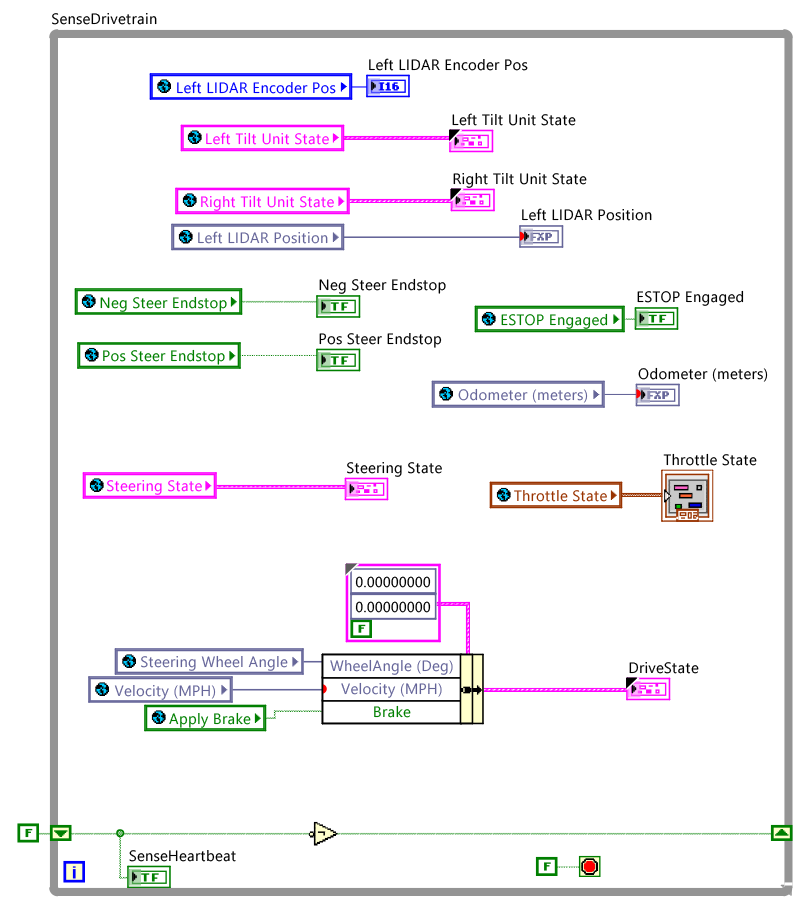
\includegraphics[scale=1.5]{Photos/sensingloop.png}
\caption{Sensing loop in the hindbrain VI}
\label{fig:sensingloop}
\end{figure} 

\noindent As shown in Figure \ref{fig:sensingloop}, the sensing loop is responsible for exposing front panel elements for the following pieces of data to the real-time code:

\begin{enumerate}
\item Left LiDAR Encoder Position: A debugging indicator that shows the encoder position of the left LiDAR in units of encoder ticks
\item Left Tilt Unit State: A cluster containing an indicator for whether the index had been found, whether the tilt unit has been told to be in initialize mode, whether there is a position error in the tilt unit and the encoder position.
\item Right Tilt Unit State: The same cluster as the left tilt unit state cluster used for the right tilt unit
\item Left LiDAR Position: Another debug indicator that shows the position of the left tilt unit in degrees after the encoder ticks have been converted to degrees
\item Negative Steer Endstop: A boolean that represents whether the negative steer angle endstop has been triggered
\item Positive Steer Endstop: A boolean that represents whether the positive steer angle endstop has been triggered
\item Estop Engaged: A boolean that represents whether either of the physical estop buttons have been triggered
\item Odometer (meters): The distance travelled by the vehicle since the code started running
\item Throttle state: A cluster containing indicators for the gas and brake pedal voltage being sent to the linear actuators for the gas and brake respectively
\item DriveState: A cluster indicating the driving state of the vehicle including the steering wheel angle in degrees, the velocity in miles per  hour and the boolean that represents whether the vehicle should apply the brakes
\item SenseHeartBeat: An indicator that simply provides a blinking light that confirms the while loop is running 
\end{enumerate}

\subsubsection{Acting Loop}

The acting loop of the FPGA hindbrain essentially performs the opposite function of the sensing loop: to provide indicators for the real-time code to pass commands or instructions down to the FPGA code. The block diagram for the acting loop shown in Figure \ref{fig:hindbrainblock} is shown zoomed in below:



\subsection{LIDAR Point Transform}

\subsubsection{Overview of the Transform Process}

The data returned by the Sick LMS290 LIDARs is in the co-ordinate frame of the LIDARs by virtue of the way in which the LIDARs take readings. In order to do useful work with the LIDAR data, the LIDAR data has to be transformed to make it iwth reference to the vehicle co-ordinate system. \\ \\
%
\noindent The transform process has two parts:

\begin{enumerate}
\item Convert each scan from polar co-ordinates to cartesian co-ordinates
\item Rotate the coordinate frames such that the frame local to the LIDAR is in the same orientation as the vehicle co-ordinates
\item Translate the coordinate frames such that the frame local to the LIDAR is translated to line up with the vehicle co-ordinate system
\end{enumerate}

\subsubsection{Constant LIDAR Transform Properties}
Based on the design and placement of the LIDAR mounts, the following properties of the LIDAR transform to t